\documentclass[a4paper,11pt,twoside]{article}
\usepackage{a4wide}
\usepackage{multirow}
\usepackage{footnote}
\usepackage{amsbsy}
\usepackage[dvips]{graphicx}
\usepackage{fancyheadings}
%\setlength{\parindent}{0in}
\setlength{\parskip}{0.05in}


% set fancy headings

\pagestyle{fancy}
\lhead[{\it \thepage}]{{\bf\it Wannier90 Tutorial}}
\chead{}
\rhead[{\bf\it Wannier90 Tutorial}]{{\it \thepage}}
\setlength{\headrulewidth}{0.2pt}
\lfoot{}
\cfoot{}
\rfoot{}
\setlength{\footrulewidth}{0pt}
\setlength{\footskip}{0.25in}
\setlength{\parindent}{0in}


\title{Wannier90: Tutorial}

\author{Version 1.0}

\begin{document}
\maketitle

{\bf Preliminaries}
Install the Wannier90 code following the instructions in the README file.
Refer to the overview of the code given in Chapter 1 of the Wannier90 User guide
and the two papers, MV\footnote{{\it Maximally localized generalized
    Wannier functions for composite energy bands}\\ N. Marzari and
  D. Vanderbilt, Phys. Rev. B 56, 12847 (1997)} 
 and SMV\footnote{{\it Maximally localized Wannier functions for entangled energy bands}\\
I. Souza, N. Marzari and D. Vanderbilt, Phys. Rev. B 65, 035109 (2002)}.


The following additional programs should be installed to visualise the output of Wannier90
\begin{itemize}
\item {\tt gnuplot} is used to plot band structures. It is 
available for many operating systems and is often installed by default on
 unix/Linux distributions\\
{\tt http://www.gnuplot.info}
\item {\tt XCrysden} is used to visualise crystal structures, Wannier functions and Fermi
surfaces. It is available for unix/Linux, Windows (using cygwin) and OSX. To correctly display
files from Wannier90 version 1.4 or later must be used.\\
{\tt http://www.xcrysden.org}
\end{itemize}



\section*{About this tutorial}

The first part of the tutorial comprises 4 examples taken from the MV and SMV papers.
All of the input files have been provided.

The second part of the tutorial covers the generation of Wannier90 input files
starting from a full electronic structure calculation. We have provided input files for the pwscf
interface to Wannier90, however these can be easily modified for other electronic structure
codes.

\cleardoublepage

\section*{1: Gallium Arsenide}

\begin{itemize}
\item{Outline: \it{Obtain and plot Wannier functions for the 4 valence bands of GaAs.}}
\item{Generation details: \it{From pwscf using norm-conserving pseudopotentials
and a 2x2x2 kpoint grid. Starting guess: 4 bond centred Gaussians.}}
\item{Directory: {\tt examples/example1/}}
\item{Input Files}
\begin{itemize}
\item{ {\tt gaas.win}  {\it The master input file}}
\item{ {\tt gaas.mmn}  {\it The overlap matrices $M_{{\bf k}}$}}
\item{ {\tt gaas.amn}  {\it Projection of the Bloch states onto a set of trial localised orbitals $A_{{\bf k}}$}}
\item{ {\tt UNK00001.1}  {\it The Bloch states in the real space unit cell. For plotting only.}}
\end{itemize}
\end{itemize}

\begin{enumerate}
\item Run the {\tt Wannier90} code to minimise the Wannier function spread
{\tt
\begin{quote}
wannier90.x gaas
\end{quote} }
Inspect the output file {\tt gaas.wout}. The total spread converges to its
minimum value after just a few iterations. Note that the geometric centre of
each Wannier function lies along a Ga-As bond, slightly closer to As
than Ga. Note also that the memory requirement for the minimisation of
the spread is very low as the Wannier functions are defined at each
kpoint by just the 4x4 unitary matrix, $U_{{\bf k}}$. 
\item Plot the Wannier Functions by adding the following keywords to the input file {\tt gaas.win}
{\tt
\begin{quote}
wannier\_plot = true
\end{quote} }
and re-running Wannier90. To visualise the Wannier functions we must explicitly represent them on
a real space grid (see User Guide Eq 2). As a consequence plotting the
Wannier functions is slower and uses more memory than the minimisation
of the spread. The 4 files that are created ({\tt gaas\_00001.xsf}, etc) can
be viewed using XCrysden 
{\tt
\begin{quote}
xcrysden --xsf gaas\_00001.xsf
\end{quote} }

For large systems plotting the Wannier functions may be time consuming
and require a lot of memory. Use the keyword {\tt wannier\_plot\_list}
to plot a subset of the Wannier functions. Eg to plot the 1st, 2nd and
7th Wannier functions use 
{\tt
\begin{quote}
wannier\_plot\_list = 1 2 7
\end{quote} }
The Wannier functions are plotted in a supercell of the unit cell. The
size of this supercell is set through the keyword {\tt
  wannier\_plot\_supercell}. The default value is 2 (corresponding to a
supercell with 8 times the unit cell volume). We recommend not using
values great than 3 as the memory and computational cost scales
cubically with  supercell size.  

Plot the 3rd Wannier function in a supercell of size 3. Choose a low
value for the isosurface (say 0.5). Can you explain what you see? 


{\it Hint} For a finite kpoint mesh the Wannier functions are in fact
periodic, where the period is related to spacing of the kpoint mesh. For
an kpoint mesh with $n$ divisions in the $ith$ direction in the
Brillouin zone the Wannier functions live in a supercell $n$ times the
unit cell. 
\end{enumerate}


\cleardoublepage



\section*{2: Lead}

\begin{itemize}
\item{Outline: \it{Obtain Wannier Functions for the 4 lowest states in Lead. Use Wannier
Interpolation to plot the Fermi Surface}}
\item{Generation Details: \it{From pwscf using norm-conserving pseudopotentials
and a 4x4x4 kpoint grid. Starting guess: atom centred sp$^3$ hybrid orbitals}}
\item{Directory: {\tt examples/example2/}}
\item{Input Files}
\begin{itemize}
\item{ {\tt lead.win}  {\it The master input file}}
\item{ {\tt lead.mmn}  {\it The overlap matrices $M_{{\bf k}}$}}
\item{ {\tt lead.amn}  {\it Projection of the Bloch states onto a set of trial localised orbitals $A_{{\bf k}}$}}
\item{ {\tt lead.eig}  {\it The Bloch eigenvalues at each kpoint. For interpolation only}}
\end{itemize}

\end{itemize}
The four lowest valence bands in lead are separated in energy from the
higher conduction states, see Figure \ref{fig:pb-bnd}. The Wannier
functions of these states have partial occupancy. Wannier functions
describing just the occupied states would exhibit very poor localisation
properties. 

\begin{enumerate}
\item Run the {\tt Wannier90} code to minimise the Wannier function spread
{\tt
\begin{quote}
wannier90.x lead
\end{quote} }
Inspect the output file {\tt lead.wout}.
\item Use Wannier interpolation to obtain the Fermi surface of
  lead. Rather than re-running the whole calculation we can use the
  unitary transformations obtained in the first calculation and restart
  from the plotting routine. Add the following keywords to the {\tt
    lead.win} file: 
{\tt
\begin{quote}
restart = plot

fermi\_energy = 5.2676

fermi\_surface\_plot = true
\end{quote} }
and re-run Wannier90. The value of the Fermi energy (5.2676 eV) was
obtained from the initial first principles calculation. The Wannier90
code calculates the band energies, through wannier interpolation, on a
dense mesh of kpoints in the Brillouin zone. The density of this grid is
controlled by the keyword {\tt fermi\_surface\_num\_points}. The default
value is 50 (ie 50$^3$ points). 
The Fermi surface file {\tt lead.bxsf} can be viewed using XCrysden
{\tt
\begin{quote}
xcrysden --bxsf lead.bxsf
\end{quote} }
\end{enumerate}

\begin{figure}[h]
\begin{center}
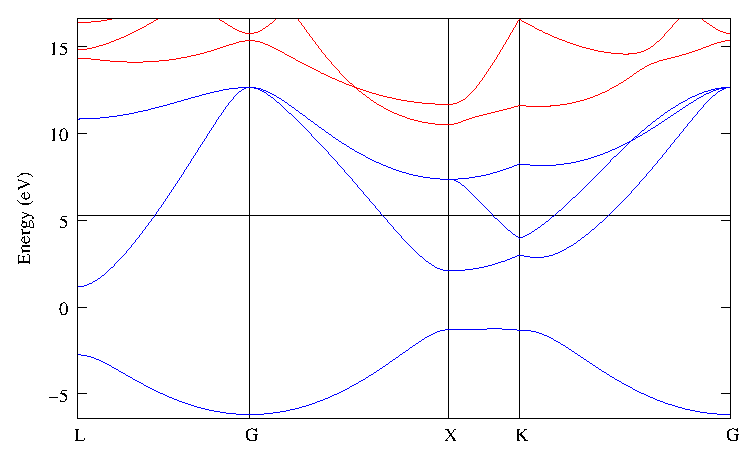
\includegraphics{lead.eps}
\caption{Band Structure of Lead showing the position of the Fermi
  level. Only the lowest 4 bands are included in the calculation.} 
\label{fig:pb-bnd}
\end{center}
\end{figure}

\cleardoublepage


\section*{3: Silicon}

\begin{itemize}
\item{Outline: \it{Obtain MLWF for the valence and low-lying conduction states of Si. Plot the interpolated band structure}}
\item{Generation Details: \it{From pwscf using norm-conserving pseudopotentials
and a 4x4x4 kpoint grid. Starting guess:  atom centred sp$^3$ hybrid orbitals}}
\item{Directory: {\tt examples/example3/}}
\item{Input Files}
\begin{itemize}
\item{ {\tt silicon.win}  {\it The master input file}}
\item{ {\tt silicon.mmn}  {\it The overlap matrices $M_{{\bf k}}$}}
\item{ {\tt silicon.amn}  {\it Projection of the Bloch states onto a set of trial localised orbitals $A_{{\bf k}}$}}
\item{ {\tt silicon.eig}  {\it The Bloch eigenvalues at each kpoint}}
\end{itemize}
\end{itemize}
The valence and lower conduction states can be represented by Wannier
Functions with sp$^3$-like symmetry. The lower conduction states are not
separated by an energy gap from the higher states. In order to form
localised Wannier function we use the disentanglement procedure
introduced in SMV. The position of the inner and outer energy windows
are shown in Figure \ref{fig:si.bnd}. 
\begin{enumerate}
\item Run the {\tt Wannier90} code.
{\tt
\begin{quote}
wannier90.x silicon
\end{quote} }
Inspect the output file {\tt silicon.wout}. The minimisation of the
spread occurs in a two step procedure. We first minimise $\Omega_{\rm
  I}$, this is the extraction of the optimal subspace in the
disentanglement procedure. We then minimise $\Omega_{\rm O}+\Omega_{{\rm
    OD}}$ 


\item Plot the Wannier Functions by adding the following commands to the input file {\tt silicon.win}
{\tt
\begin{quote}
restart = plot

bands\_plot = true
\end{quote} }
and re-running Wannier90. The files {\tt silicon\_band.dat} and {\tt silicon\_band.gnu} are created.
To plot the band-structure using gnuplot
\smallskip
{\tt
\begin{quote}
myshell> gnuplot

gnuplot> load `silicon\_band.gnu'
\end{quote} }
The kpoint path for the bandstructure interpolation is set in the {\tt kpoint\_path} block. Try plotting along different paths.
\end{enumerate}

\begin{figure}[h]
\begin{center}
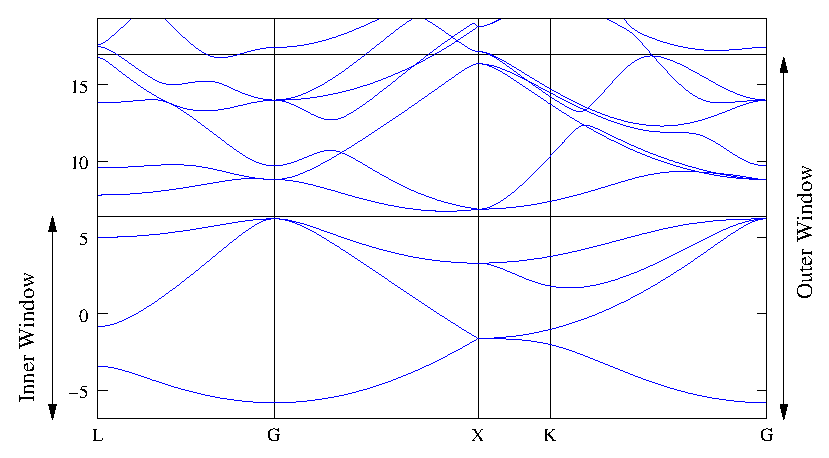
\includegraphics{si.eps}
\caption{Band Structure of Silicon showing the position of the outer and inner energy windows.}
\label{fig:si.bnd}
\end{center}
\end{figure}

\cleardoublepage


\section*{4: Copper}

\begin{itemize}
\item{Outline: \it{Obtain MLWF to describe the states around the Fermi-level in Copper}}
\item{Generation Details: \it{From pwscf using ``ultrasoft'' pseudopotentials
and a 4x4x4 kpoint grid. Starting guess: 5 atom centred `d' orbital and two `s' orbitals centred on 
one of each of the two tetrahedral interstices.}}
\item{Directory: {\tt examples/example4/}}
\item{Input Files}
\begin{itemize}
\item{ {\tt copper.win}  {\it The master input file}}
\item{ {\tt copper.mmn}  {\it The overlap matrices $M_{{\bf k}}$}}
\item{ {\tt copper.amn}  {\it Projection of the Bloch states onto a set of trial localised orbitals $A_{{\bf k}}$}}
\item{ {\tt copper.eig}  {\it The Bloch eigenvalues at each kpoint}}
\end{itemize}

\end{itemize}

\begin{enumerate}
\item Run the {\tt Wannier90} code to minimise the Wannier function spread
{\tt
\begin{quote}
wannier90.x copper
\end{quote} }
Inspect the output file {\tt copper.wout}. 

\item Plot the Fermi surface, it should look familiar! The Fermi energy is at 12.2103eV.

\item Plot the interpolated band structure. A suitable path in kspace is
\smallskip
{\tt
\begin{quote}
begin kpoint\_path

G 0.00  0.00  0.00    X 0.50  0.50  0.00

X 0.50  0.50  0.00    W 0.50  0.75  0.25

W 0.50  0.75  0.25    L 0.00  0.50  0.00

L 0.00  0.50  0.00    G 0.00  0.00  0.00

G 0.00  0.00  0.00    K 0.00  0.50 -0.50
 
end kpoint\_path
\end{quote} }
\end{enumerate}
Investigate the effect of the outer and inner energy window on the interpolated bands.



\begin{figure}[h]
\begin{center}
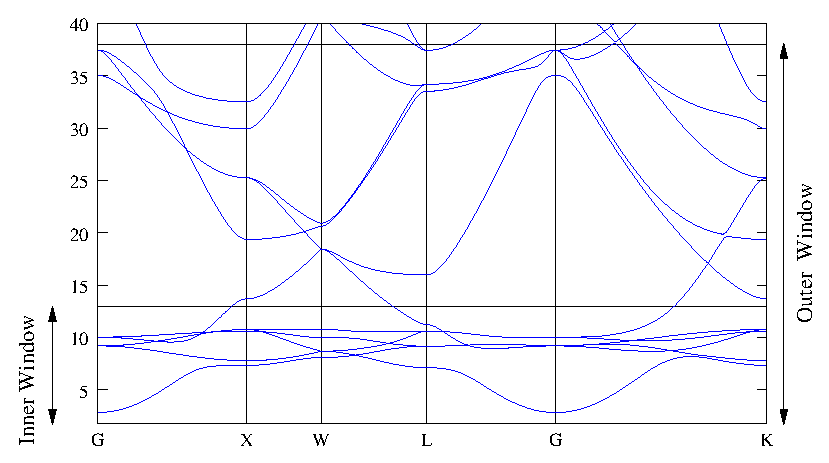
\includegraphics{cu.eps}
\caption{Band Structure of Copper showing the position of the outer and inner energy windows.}
\label{fig:cu-bnd}
\end{center}
\end{figure}

\cleardoublepage

\section*{PWSCF Examples}

A fully featured interface between Wannier90 and Pwscf will be available as part of the 
next Quantum Espresso release. Before that time it can be downloaded as part of the
pwscf development distribution. Use the following commands to download a copy from the
pwscf cvs server (bash shell):
\begin{verbatim}
export CVS_RSH=ssh
export CVSROOT=:pserver:cvsanon@democritos.sissa.it:/home/cvs
cvs login  (The password is: cvsanon)
cvs checkout pwscf
\end{verbatim}

\subsection*{Diamond}
\begin{itemize}
\item{Outline: \it{Obtain MLWF for the occupied state of Diamond}}
\item{Directory: {\tt examples/example5/}}
\item{Input Files}
\begin{itemize}
\item{ {\tt diamond.scf}  {\it Pwscf input file for ground state calculation}}
\item{ {\tt diamond.nscf}  {\it Pwscf input file to obtain Bloch states on a uniform grid}}
\item{ {\tt diamond.pw2wan}  {\it Input file for pw2wannier90}}
\item{ {\tt diamond.win}  {\it Wannier90 input file}}
\end{itemize}

\end{itemize}

\begin{enumerate}
\item Run pwscf to obtain the ground state of Diamond\\
{\tt pw.x < diamond.scf > scf.out}

\item Run pwscf to obtain the Bloch states on a uniform kpoint grid\\
{\tt pw.x < diamond.nscf > nscf.out}

\item Run Wannier90 to generate a list of the required overlaps (written
  into the {\tt diamond.nnkp} file).\\ 
{\tt wannier90.x -pp diamond}

\item Run pw2wannier to compute the overlap between Bloch states and the
  projections for the starting guess (written in the {\tt diamond.mmn} and {\tt diamond.amn} files).\\ 
{\tt pw2wannier90.x < diamond.pw2wan > pw2wan.out}

\item Run Wannier90 to compute the Wannier functions.\\
{\tt wannier90.x diamond}

\end{enumerate}

\subsection{Still to write up}

\begin{enumerate}

\item Silane

\item Iron (spin up channel)

\item Maybe MnO

\end{enumerate}




\end{document}
